\documentclass[12pt,a4paper,twoside]{article}
\usepackage{labor}
\begin{document}

%fill for cover and header creation
\newcommand\laboratorynumber{2}
\title{Halbleiterdiode}
\newcommand\supervisor{Ditlbacher, Harald}
\newcommand\groupnumber{42}

\newcommand\participantonelastname{Eisner}
\newcommand\participantonefirstname{Nico}
\newcommand\participantoneid{12214121}
\newcommand\participanttwolastname{Waldl}
\newcommand\participanttwofirstname{Philip}
\newcommand\participanttwoid{12214120}
\author{\participantonelastname \ \& \participanttwolastname}

\newcommand\degreeid{UB 033 678}
\newcommand\semester{23WS}
\date{15.12.2023}

%select correct course title
%\newcommand\coursetitle{Einführung in die \\ physikalischen Messmethoden}
%\newcommand\coursetitle{Laborübungen 1: \\ Mechanik und Wärme}
\newcommand\coursetitle{Laborübungen 2: \\ Elektrizität, Magnetismus, Optik}
%\newcommand\coursetitle{Fortgeschrittenen Praktikum 1: \\ Technische Physik}
%\newcommand\coursetitle{Fortgeschrittenen Praktikum 2: \\ Allgemeine Physik}

%\begin{titlepage}
   \begin{center}
       \begin{figure}[H]
            \begin{minipage}[h]{30mm}
                \centerline{
\includegraphics[height=15mm]{cover_nudes/tugraz.png}}
            \end{minipage}
            \hfill
            \begin{minipage}[h]{30mm}
                \centerline{
\includegraphics[height=15mm]{cover_nudes/nawi_graz.png}}
            \end{minipage}
            \hfill
            \begin{minipage}[h]{30mm}
                \centerline{
\includegraphics[height=15mm]{cover_nudes/uni-graz.png}}
            \end{minipage}
        \end{figure}
        
        \large{\emph{Institut für Experimentalphysik der Technischen Universität Graz \\
        \& Institut für Physik der Universität Graz}} \\
        \vspace{5mm}
        
        {\Huge \textbf{\coursetitle}}
        \vspace{5mm}
        
        {\huge \laboratorynumber: \thetitle}
    \end{center}
    
    \vfill
    
    \begin{table}[H]
        \LARGE
        \centering
        \begin{tabular}{r l}
            Betreuer:       & \supervisor \\
            Gruppennummer:  & \groupnumber \\
            \\
            Name:           & \participantonelastname, \participantonefirstname \\
            Matrikelnummer: & \participantoneid \\
            Name:           & \participanttwolastname, \participanttwofirstname \\
            Matrikelnummer: & \participanttwoid \\
            \\
            Kennzahl:       & \degreeid \\
            Datum:          & \semester \ | \thedate
        \end{tabular}
    \end{table}
    \vspace{4cm}
\end{titlepage}
\clearpage
\setcounter{page}{1}

%\maketitle %short title alternative

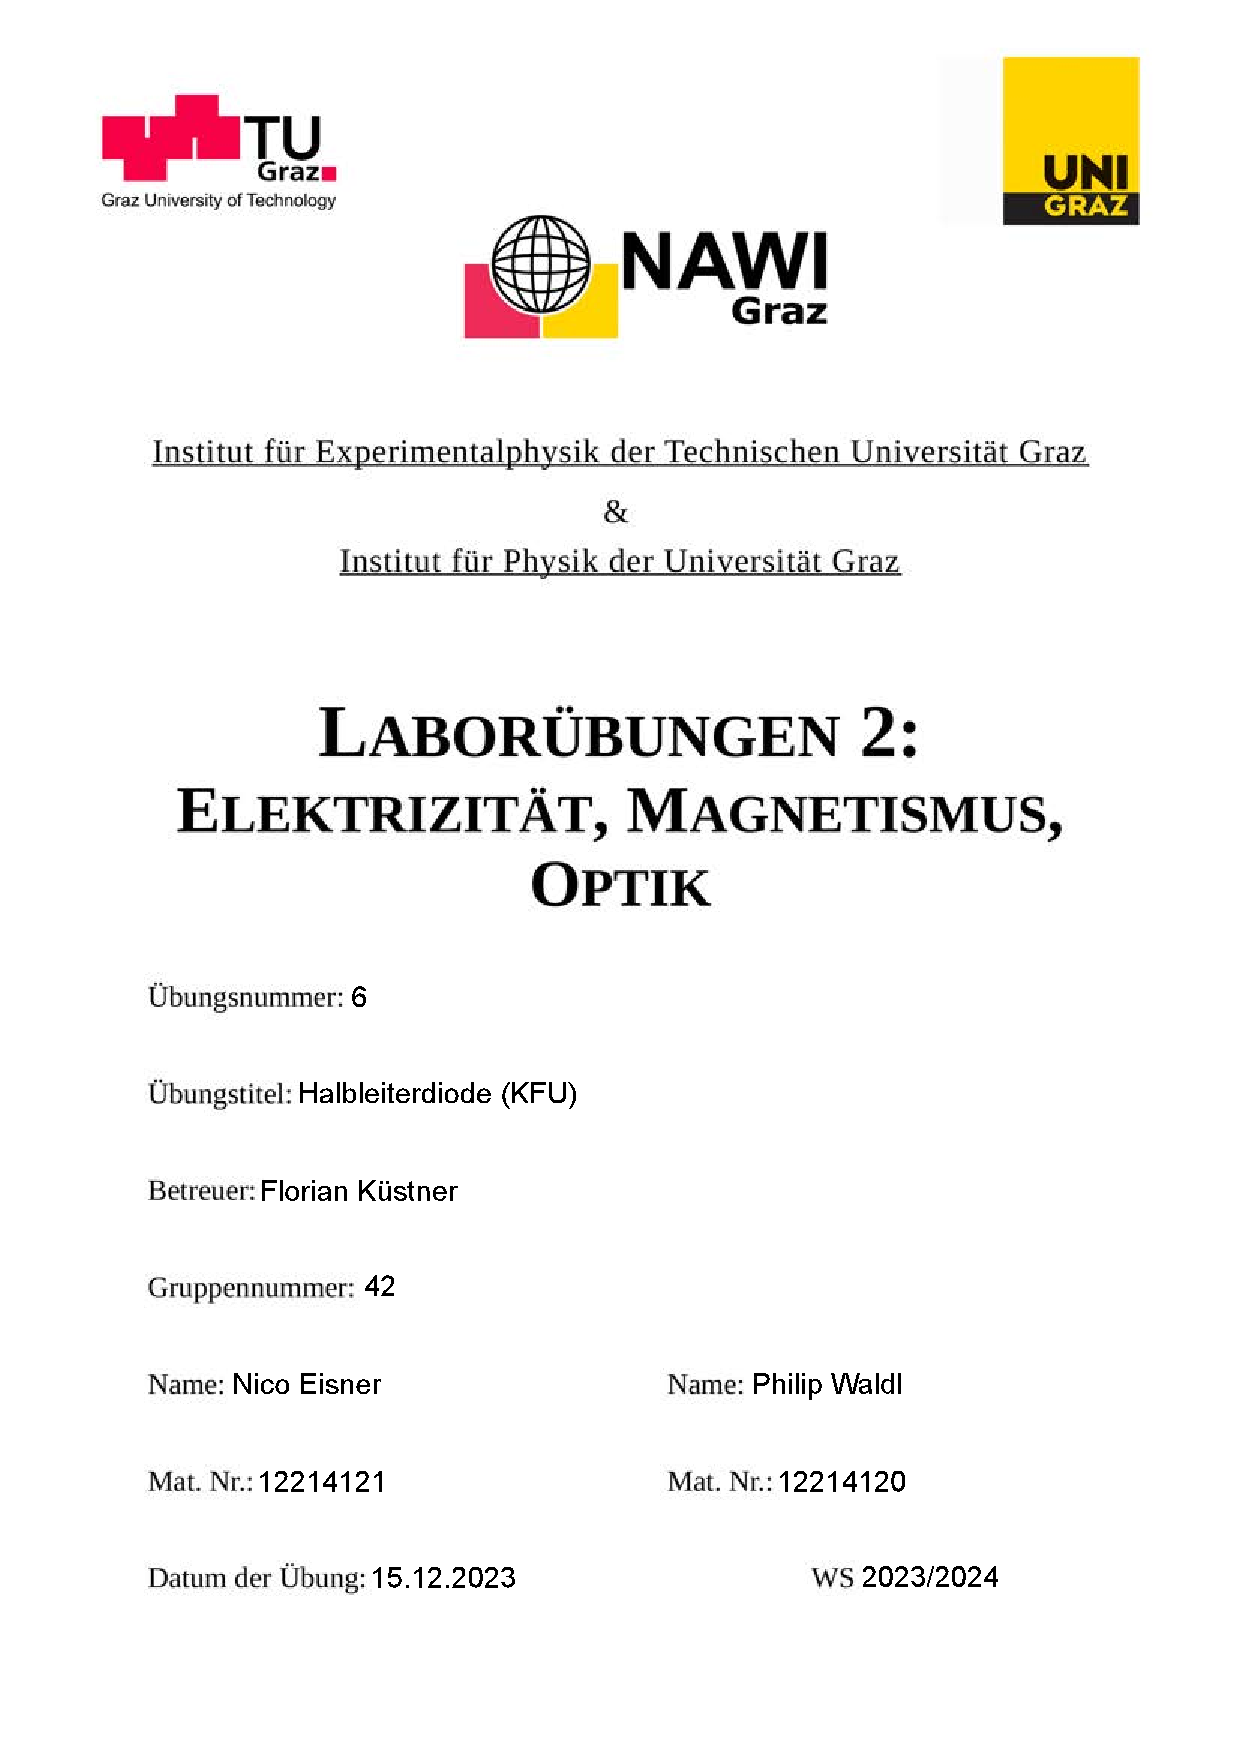
\includepdf[pages={1}]{../Deckblätter/Deckblatt_Halbleiterdiode.pdf}

\tableofcontents
\newpage

\section{Aufgabenstellung} %jo beschreibn wos gmocht host ------------------------------
Das Experiment Halbleiterdiode besteht aus drei Teilaufgaben. 
\\
In der ersten Teilaufgabe gilt es die Strom-Spannungs Charakteristik einer Gleichrichterdiode in Durchlassrichtung sowie in Sperrrichtung zu bestimmen. 
\\
Im zweiten Teil wird die Strom-Spannungs Charakteristik einer Zenerdiode in Durchlassrichtung und Sperrrichtung bestimmt. 
\\
Im dritten und letzten Teil werden Spannungs- und Stromverläufe in einer Einweg- Gleichrichterschaltung mit unterschiedlichen Glättungskondensatoren sowie mit Belastungswiderständen untersucht. 
\\
\\
Alle Informationen und Methodiken wurden uns von der Technischen Universität bereitgestellt \cite{teachcenter2}. 


\section{Voraussetzungen \& Grundlagen} %Grundlagen erklären, Formeln mit erklärung
Um mit dem Experiment beginnen zu können gilt es erst zu erklären, was ein Halbleiter ist. 
\\
Es gibt drei arten der elektrischen Leitfähigkeit. Leitern, Nichtleitern und Halbleitern. Mithilfe des quantenmechanischen Bändermodells lässt sich die Leitfähigkeit beschreiben. 
Dieses besteht aus den zwei Energiebändern (Leitungsband und Valenzband) und der Bandlücke. Valenzelektronen befinden sich im Valenzband und dienen als Ladungsträger. Im Grundzustand ist das Leitungsband nicht mit Elektronen besetzt. 
Zwischen diesen befindet sich bei Halbleitern und Nichtleitern die Bandlücke. 

\begin{figure}[H]
    \centering
    \includegraphics[width=0.6\linewidth,]{nudes/bändermodell.jpg}
    \caption{Bändermodell eines Nichtleiters, Halbleiters und Leiters. Entnommen aus Skriptum Halbleiterdiode Abbildung 7. \cite{teachcenter2}}
    \label{fig:Bändermodell}
\end{figure}

\noindent
Bei Leitern existiert keine Bandlücke. Das Valenzband ist nicht voll mit Elektronen besetzt oder es überlappt mit dem Leitungsband. Diese Zustände treffen gleichzeitig zu. 
Bei Nichtleitern ist zwischen Valenzband und Leitungsband die Bandlücke. Das Valenzband ist voll mit Elektronen, diese können aber nicht zum Leitungsband gelangen. 
Bei Halbleitern ist die Bandlücke sehr klein im Gegensatz zu Nichtleitern. Bei Raumtemperatur können Elektronen vom Valenzband in das Leitungsband gelangen. 
Dadurch hinterlässt jedes in das Leitungsband übergetretene Elektron ein Loch, welches durch andere Elektronen besetzt wird. 
\\
Da die Elektronen aber wieder in dieses Loch zurückfallen würden, ist die Eigenleitfähigkeit dieser Halbleiterelemente nicht verwertbar. 
\\
\\
Durch das einbringen fremder Atome in den Halbleiterkristall lässt sich die Leitfähigkeit ändern. Halbleiter bestehen meißt aus Silizium oder Germanium. 
Bei Silizium handelt es sich um 4-wertige Valenzelelektronen. Durch einbringen eines 3-wertigen oder 5-wertigen Atomes lässt sich die Leitfähigkeit gezielt verändern. 

\begin{figure}[H]
    \centering
    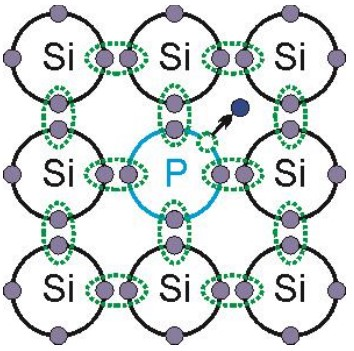
\includegraphics[width=0.3\linewidth,]{nudes/n-dot.jpg}
    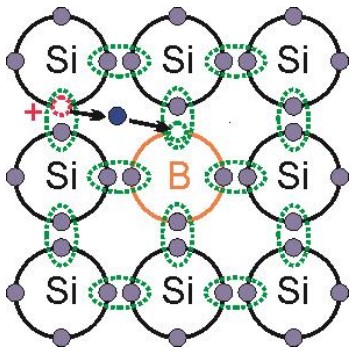
\includegraphics[width=0.3\linewidth,]{nudes/p-dot.jpg}
    \caption{n-Dotierter Kristall (links) und p-Dotierter Kristall (rechts). Bei dem n-Dotierten Kristall wird Phosphor eingebracht und bei dem p-Dotierten wird Bor eingebracht. Entnommen aus Skriptum Halbleiterdiode Abbildung 8 und 9. \cite{teachcenter2}}
    \label{fig:n und p dotiert}
\end{figure}

\noindent
Bringt man in die Kristallstruktur ein 5-wertiges Dotierelement ein, so spricht man von n-Dotierung. Dieses fünfte Elektron ist dabei frei beweglich. 
Bringt man ein 3-wertiges Dotierelement ein, so spricht man von p-Dotiertung. Dieses entstandene Loch kann ein Außenelektron aufnehmen. 
Bei einen pn-Übergang ist dies genau der Fall. Dieser ist der Übergangsbereich unterschiedlich dotierter Halbleiterkristalle. 
Elektronen des n-Kristalls wandern zuu den Löchern des p-Kristalls. Löcher des p-Kristalls wandern zu den Elektronen des n-Kristalls. 
Durch diesen Vorgang entsteht ein elektrisches Feld. Der Halbleiter ist nichtmehr elektrisch neutral und die Kraft, welche das el. Feld erzeugt wirkt auf die verbleibenden Ladungsträger. 
\\
\\
Verpackt man eine p-n Übergang in ein Gehäuse und versorgt ihn mit Anschlüssen erhält man eine Diode. 

\begin{figure}[H]
    \centering
    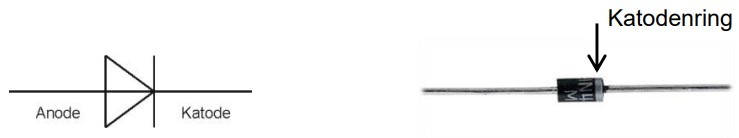
\includegraphics[width=0.6\linewidth,]{nudes/diode.jpg}
    \caption{Schaltbild und Foto einer Diode. Entnommen aus Skriptum Halbleiterdiode Abbildung 15. \cite{teachcenter2}}
    \label{fig:Diode}
\end{figure}

\noindent
Um aus einer Spannung $U$ und einem Widerstand $R$ einen Strom $I$ zu berechnen benötigt man das Ohm'sche Gesetzt, was besagt: 

\begin{equation}
    \label{eq:ohmsche}
    \centerline{$I=\frac{U}{R}$ \\ $\Delta I = \vert \frac{\partial I}{\partial U} * \Delta U \vert + \vert \frac{\partial I}{\partial R} * \Delta R \vert $}
\end{equation}

\noindent
Um die Spannung $U_R$ an einen Widerstand zu bestimmen, benötigt man die Eingangsspannung $U_E$ sowie die Spannung an der Diode $U_{D1}$. 
\\
Es gilt dann: 

\begin{equation}
    \label{eq:ur1}
    \centerline{$U_{R1}= U_E - U_{D1}$ \\ $\Delta U_{R1} = \vert \frac{\partial U_{R1}}{\partial U_E} * \Delta U_E \vert + \vert \frac{\partial U_{R1}}{\partial U_{D1}} * \Delta U_{D1} \vert $}
\end{equation}

\section{Versuchsanordnung} %mit skizze kurz beschreiben ------------------------------
Der Versuch wird auf dem Steckbrett aufgebaut und durch mehrere Messgeräte wie Multimeter und Oszilloskope ergänzt. 

\begin{figure}[H]
    \centering
    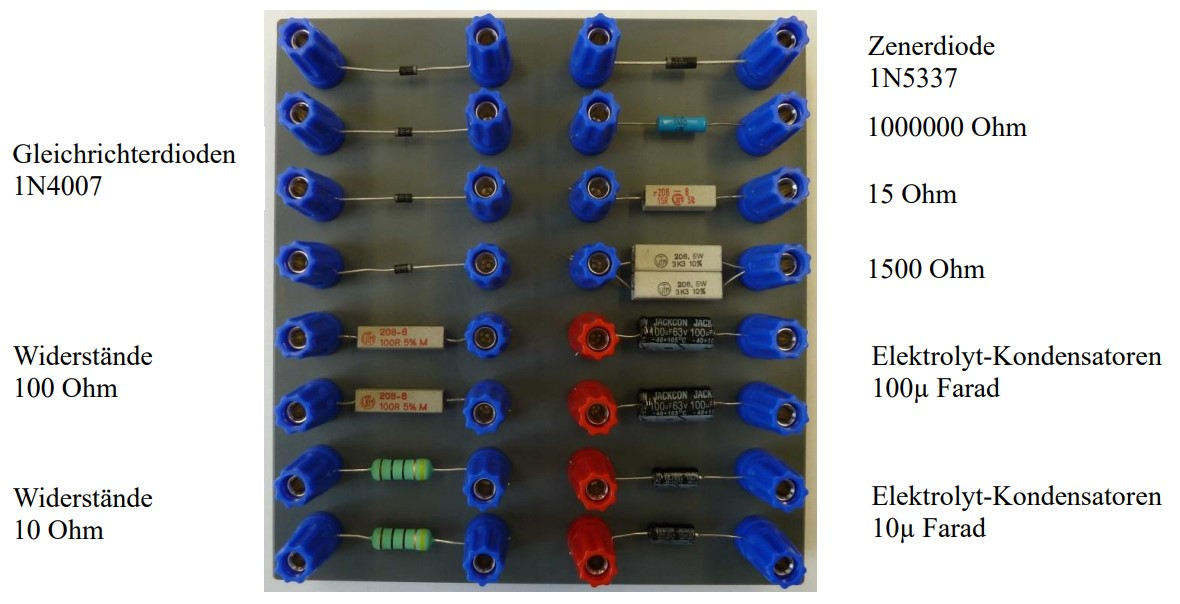
\includegraphics[width=0.6\linewidth]{nudes/steckbrett.jpg}
    \caption{Steckbrett mit Bauteilen. Entnommen aus Skriptum Halbleiterdiode Abbildung 1. \cite{teachcenter2}}
    \label{fig:Steckbrett}
\end{figure}

\subsection{Teil 1}
Im ersten Teil wird die Strom-Spannungskennlinie der Gleichrichterdiode in Durchlassrichtung bestimmt. Der Aufbau sieht dabei wiefolgt aus. 

\begin{figure}[H]
    \centering
    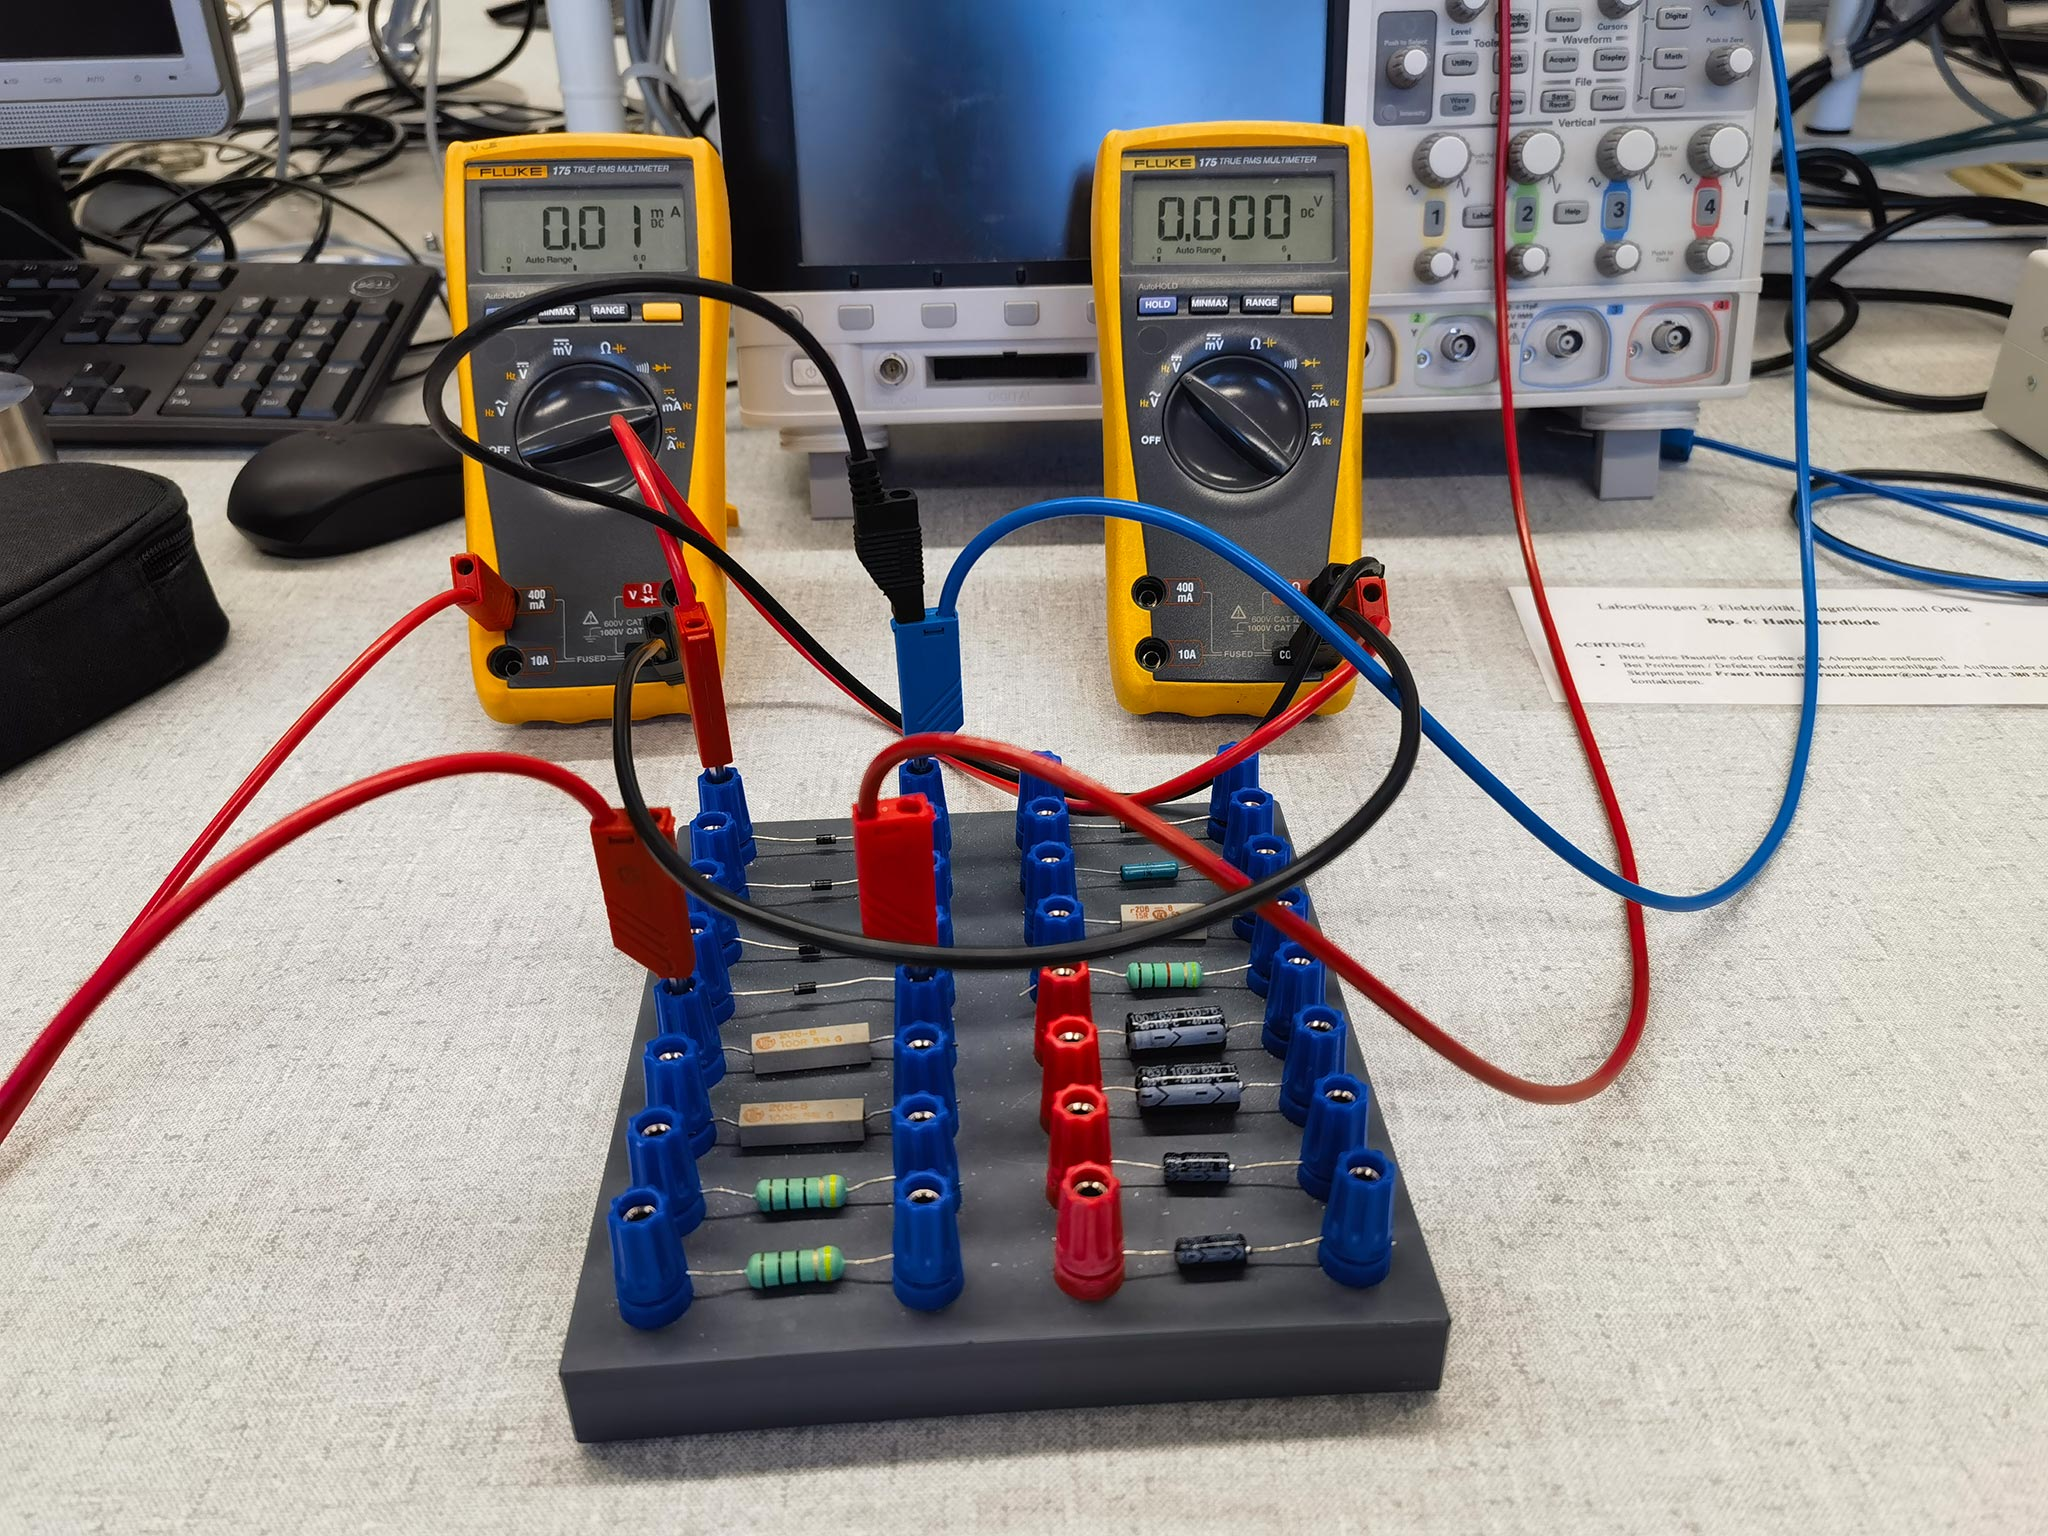
\includegraphics[width=0.4\linewidth]{nudes/1a.jpg}
    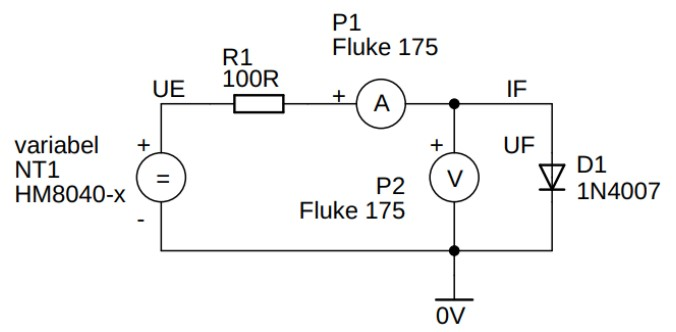
\includegraphics[width=0.4\linewidth]{nudes/aufbau1a schaltplan.jpg}
    \caption{Schaltbild (links) und Aufbau (rechts) Teil 1. Schaltbild entnommen aus Skriptum Halbleiterdiode Abbildung 1. \cite{teachcenter2}}
    \label{fig:aufbau 1a}
\end{figure}

\noindent
Das gleiche wird anschließend für die Gleichrichterdiode in Sperrichtung wiederholt.

\begin{figure}[H]
    \centering
    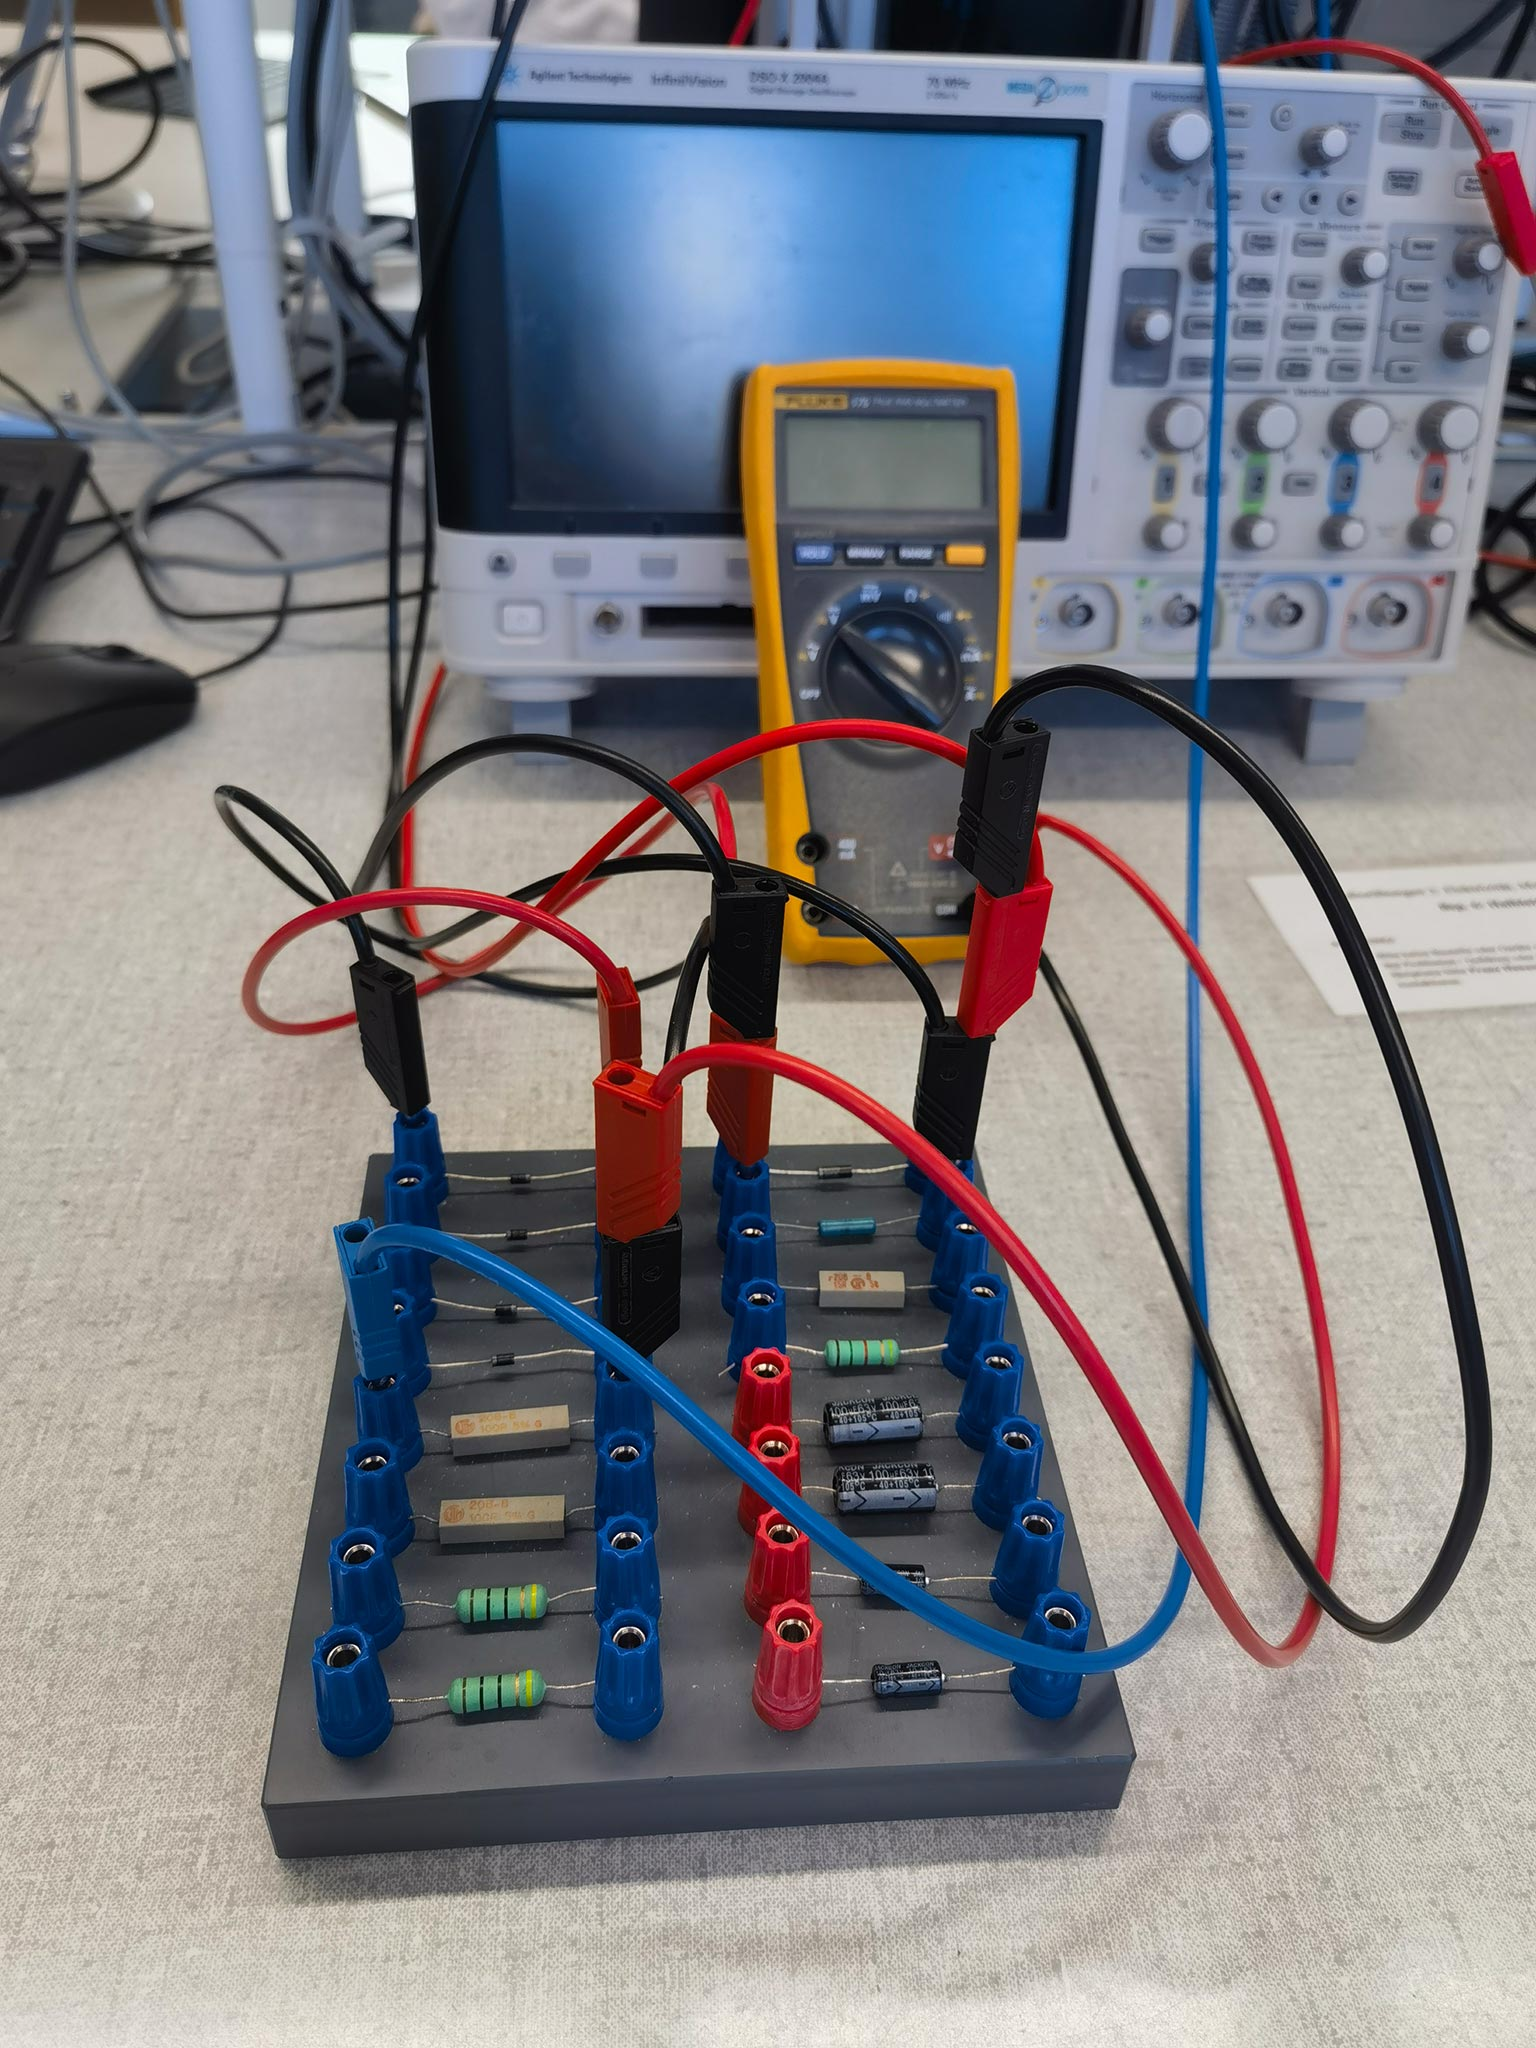
\includegraphics[width=0.4\linewidth]{nudes/1b.jpg}
    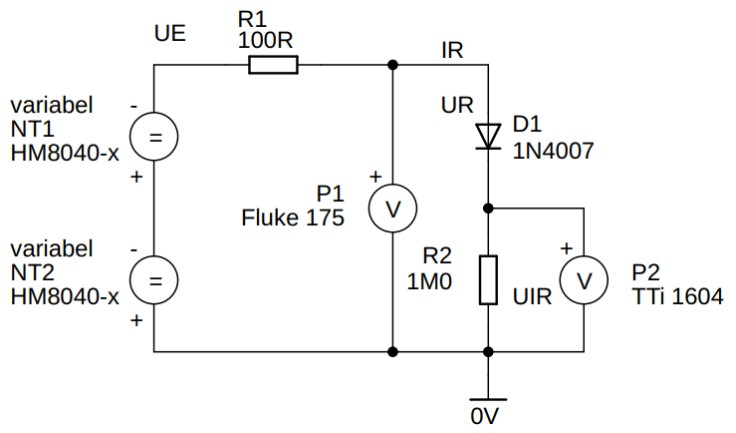
\includegraphics[width=0.4\linewidth]{nudes/aufbau1b schaltplan.jpg}
    \caption{Schaltbild (links) und Aufbau (rechts) Teil 1. Schaltbild entnommen aus Skriptum Halbleiterdiode Abbildung 1. \cite{teachcenter2}}
    \label{fig:aufbau 1b}
\end{figure}

\subsection{Teil 2}
Im zweiten Teil wird die Strom-Spannungskennlinie einer Zenerdiode aufgenommen. 

\begin{figure}[H]
    \centering
    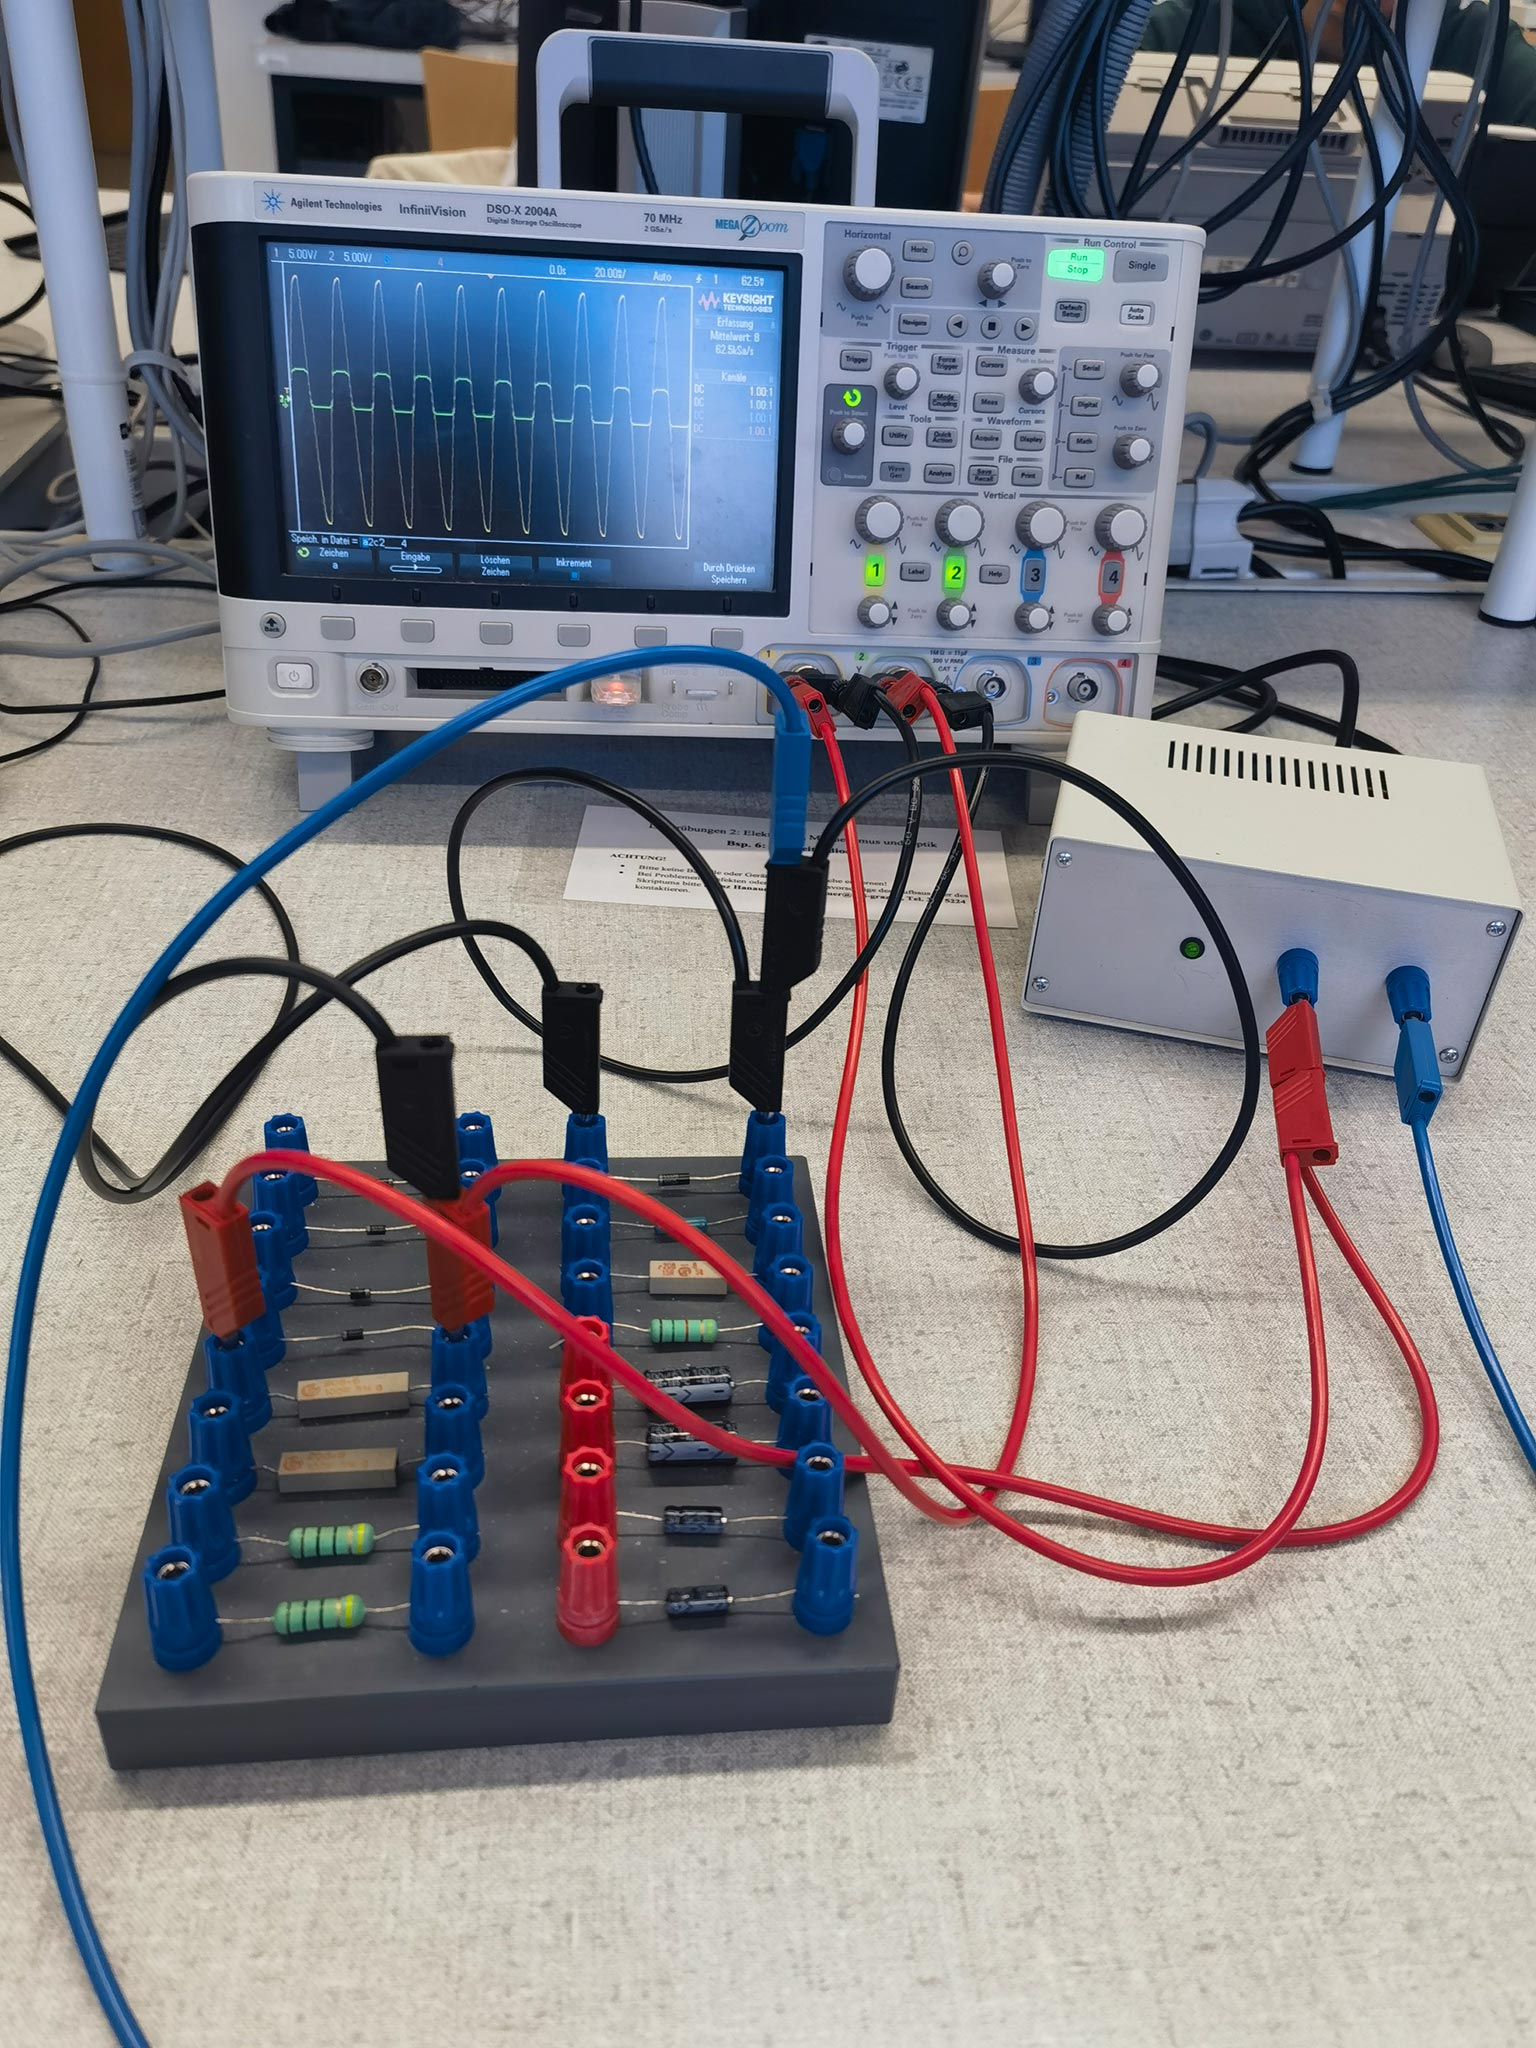
\includegraphics[width=0.4\linewidth]{nudes/2.jpg}
    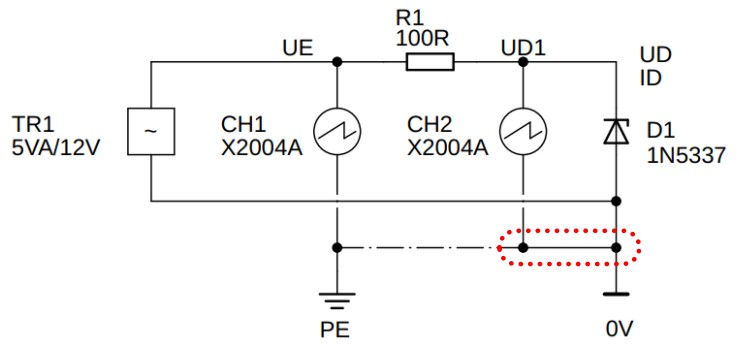
\includegraphics[width=0.4\linewidth]{nudes/aufbau2 schaltplan.jpg}
    \caption{Schaltbild (links) und Aufbau (rechts) Teil 2. Schaltbild entnommen aus Skriptum Halbleiterdiode Abbildung 1. \cite{teachcenter2}}
    \label{fig:aufbau 2}
\end{figure}

\subsection{Teil 3}
Im dritten Teil wird die grafische Darstellung der Verläufe von Strom und Spannung bestimmt. 

\begin{figure}[H]
    \centering
    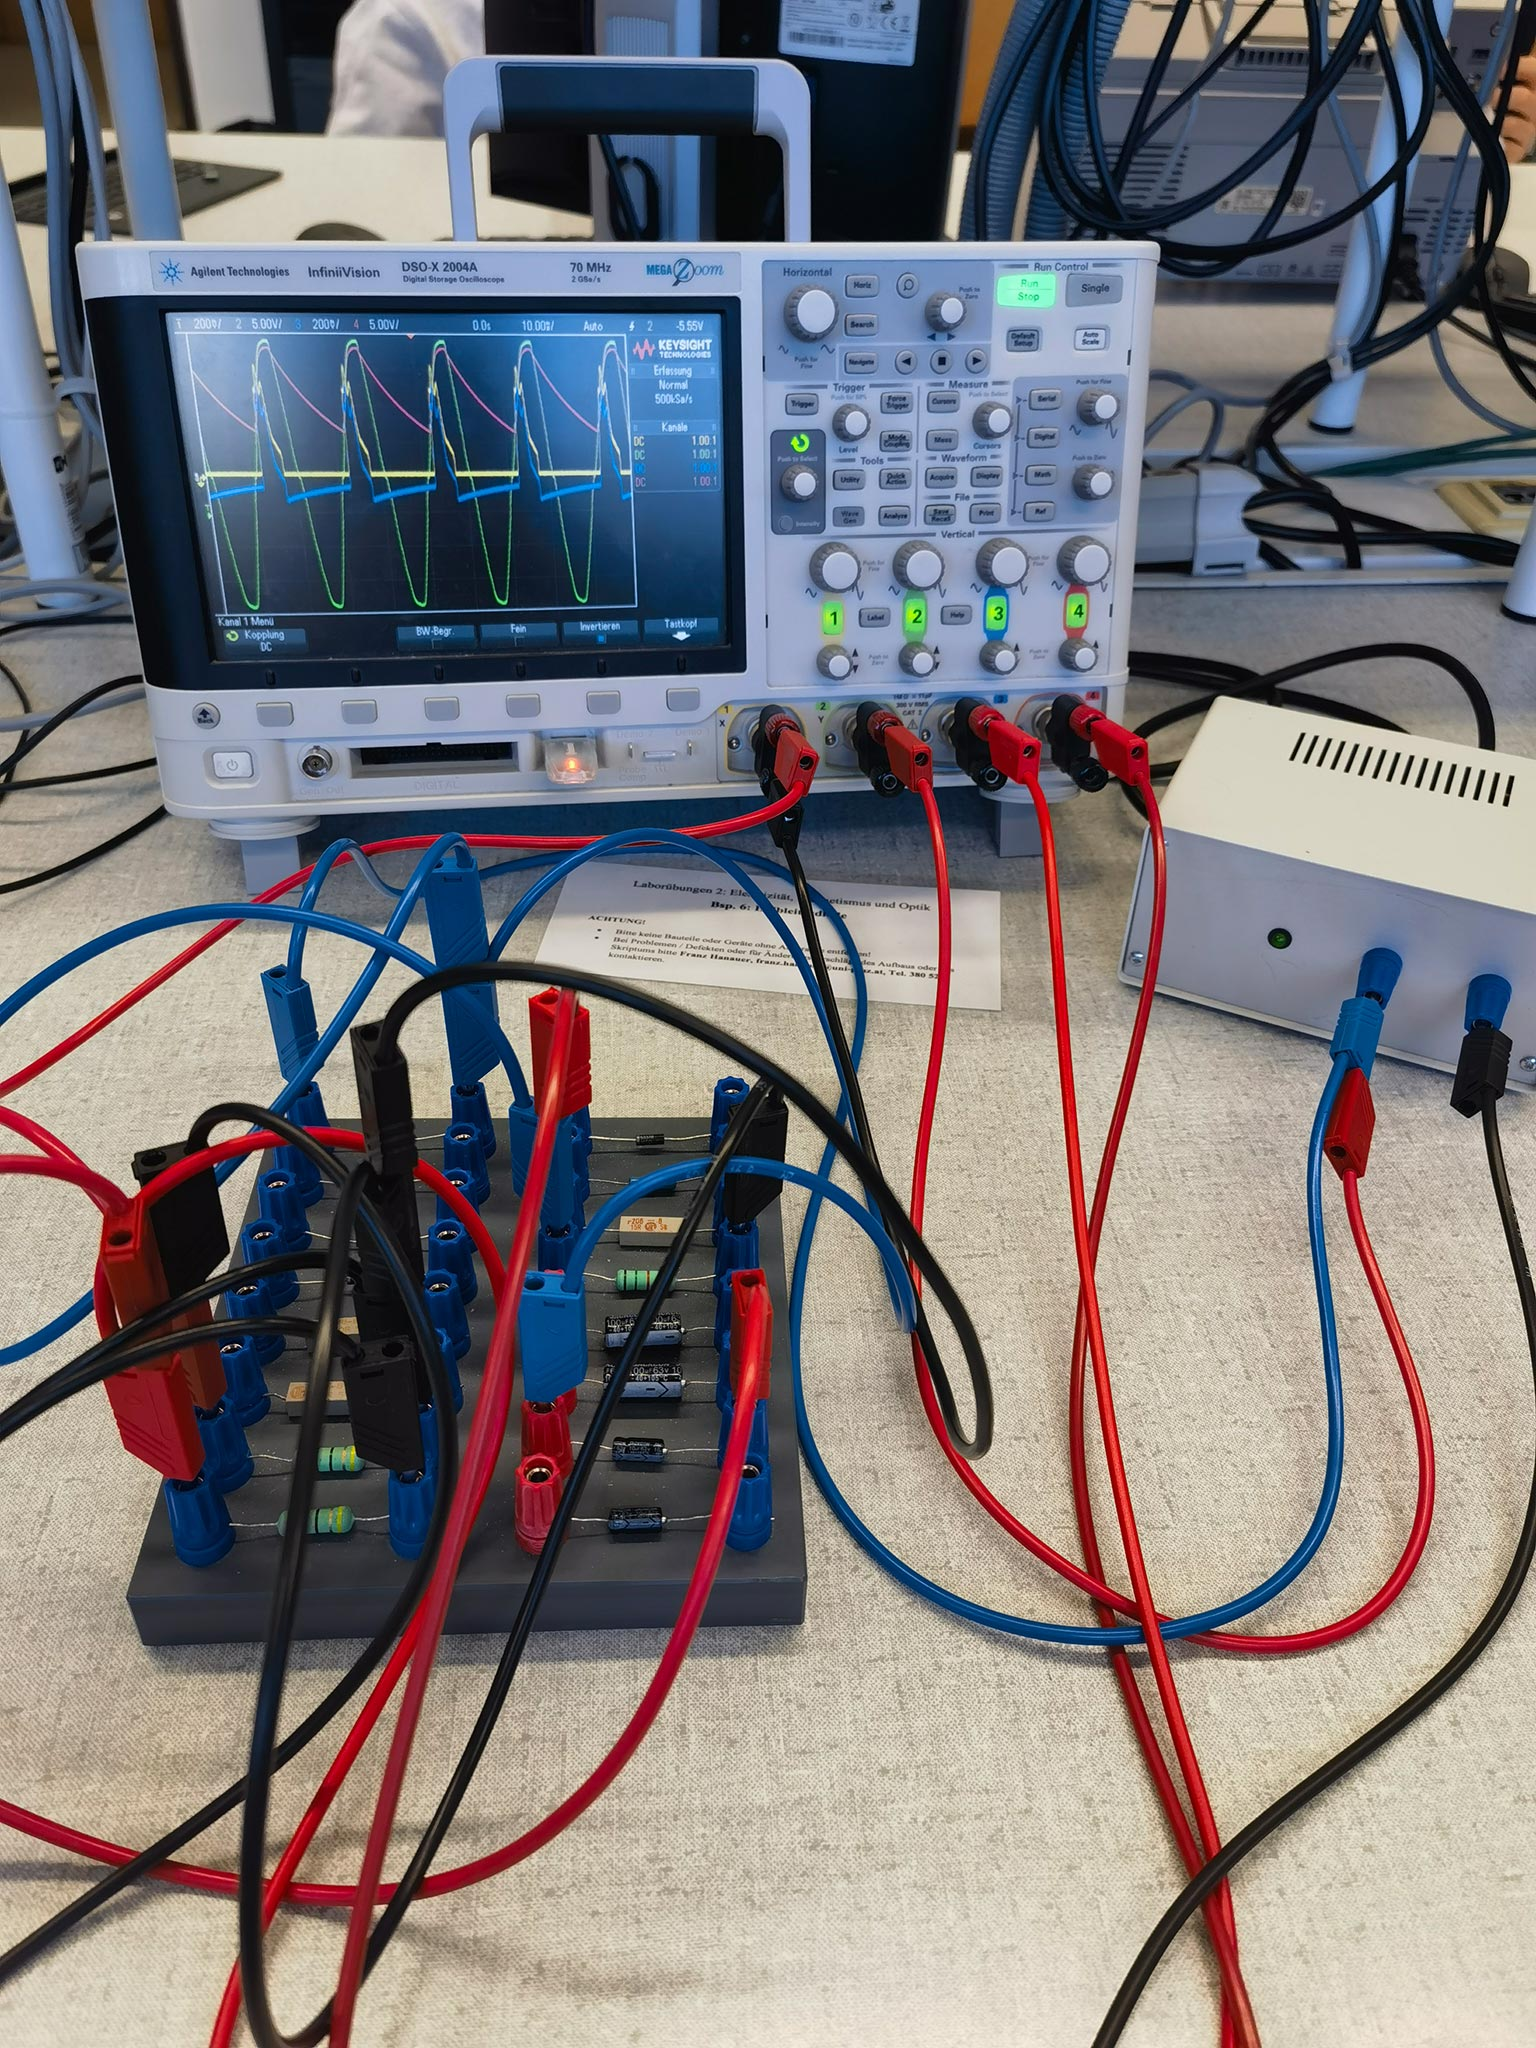
\includegraphics[width=0.4\linewidth]{nudes/3.jpg}
    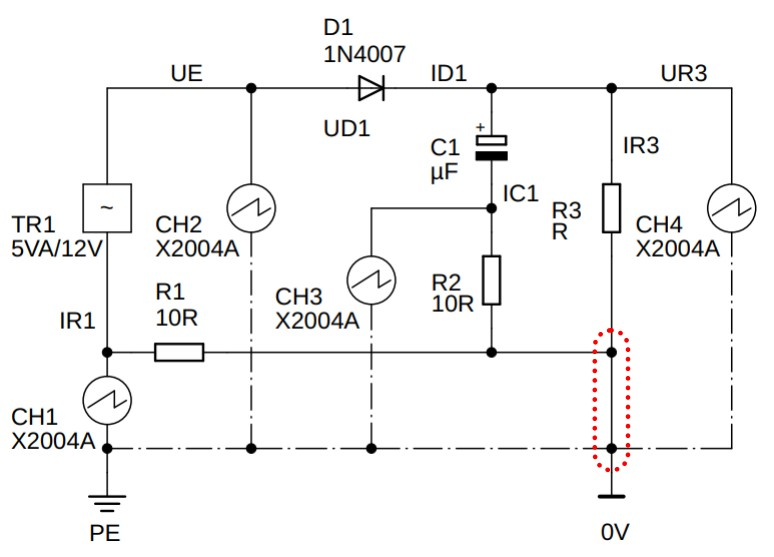
\includegraphics[width=0.4\linewidth]{nudes/aufbau3 schaltplan.jpg}
    \caption{Schaltbild (links) und Aufbau (rechts) Teil 3. Schaltbild entnommen aus Skriptum Halbleiterdiode Abbildung 1. \cite{teachcenter2}}
    \label{fig:aufbau 3}
\end{figure}

\section{Geräteliste} %jo holt a listn ------------------------------

    \begin{table}[H]
        \centering
        \caption{Im Versuch verwendete Geräte und Utensilien.}
        \label{tab:geraete}
        \begin{tabular}{| l | l | l |}
            \hline
            Gerät   & Gerätenummer  & Unsicherheit \\
            \hline
            Steckbrett & {n.a} & {n.a} \\
            Multimeter & Fluke 175 & $\pm (0.15\% + 2 dig.) V$ \\
            & & $\pm (1.0\% + 3 dig.) A$ \cite{fluke}\\
            Multimeter & TTI 1604 & $\pm (0.08\% + 4 dig.) V$ \cite{TTI} \\
            Power Supply & HM8040-3 & {n.a}\\
            Trafo & {n.a} & {n.a}\\
            Oszilloskop & Agilent Tech. DSO-X 2004A & {n.a}\\
            \hline
        \end{tabular}
    \end{table}


\section{Versuchsdurchführung \& Messergebnisse} %nachvollziehbar und klar dargestellt ------------------------------

\subsection{Teil 1}
Im ersten Teil werden die Versuche nach den Abbildungen \ref{fig:aufbau 1a} und \ref{fig:aufbau 1b} aufgebaut. 
Die Aufgabe besteht darin, die Strom-Spannungs Charakteristik einer SI-Gleichrichterdiode in Durchlassrichtung und Sperrrichtung zu bestimmen. 
Die Widerstände $R_1 = (100 \pm 1) \Omega$ und $R_2 = (1*10^6 \pm 1*10^3) \Omega$ werden zuvor mit dem Messgerät kontrolliert (Unsicherheiten implizit angenommen). 
\\
\\
Es werden für die Druchlassrichtung der Druchlassstrom $I_F$ sowie die Durchlassspannung $U_F$ gemessen. Die Messungen erfolgen mit den Fluke 175 Messgeräten. 
Am Netzteil wählt man eine Spannung im bereich 0-20 V. Durch den Widerstand R1 (Abb. \ref{fig:aufbau 1a}) wird der Durchlassstrom auf max. 200 mA begrenzt. 
Die Unsicherheit der Eingangsspannung $U_{ein}$ ist die Ableseunsicherheit. 

\begin{table}[H]
    \centering
    \caption{Messwerte der SI-Gleichrichterdiode in Durchlassrichtung. }
    \label{tab:mess1a}
    \begin{tabular}{| l | l | l | l |}
        \hline
        Nr. & $U_{ein} \pm 0.1$ / V & $U_F$ / V & $I_F$ / mA \\
        \hline
        1  & 0.1  & -0.118 $\pm$ 0.003 & 0.01 $\pm$ 0.03 \\
        2  & 0.2  & -0.291 $\pm$ 0.003 & 0.01 $\pm$ 0.03 \\
        3  & 0.3  & -0.356 $\pm$ 0.003 & 0.01 $\pm$ 0.03 \\
        4  & 0.4  & -0.482 $\pm$ 0.003 & 0.12 $\pm$ 0.04 \\
        5  & 0.5  & -0.531 $\pm$ 0.003 & 0.35 $\pm$ 0.04 \\
        6  & 0.6  & -0.569 $\pm$ 0.003 & 0.76 $\pm$ 0.05 \\
        7  & 0.7  & -0.605 $\pm$ 0.003 & 1.57 $\pm$ 0.06 \\
        8  & 0.8  & -0.629 $\pm$ 0.003 & 2.54 $\pm$ 0.07 \\
        9  & 0.9  & -0.641 $\pm$ 0.003 & 3.21 $\pm$ 0.08 \\
        10 & 0.10 & -0.647 $\pm$ 0.003 & 3.64 $\pm$ 0.09 \\
        11 & 0.11 & -0.662 $\pm$ 0.003 & 4.93 $\pm$ 0.11 \\
        12 & 0.12 & -0.672 $\pm$ 0.004 & 5.92 $\pm$ 0.12 \\
        13 & 0.13 & -0.681 $\pm$ 0.004 & 7.09 $\pm$ 0.14 \\
        14 & 0.14 & -0.685 $\pm$ 0.004 & 7.52 $\pm$ 0.15 \\
        \hline
    \end{tabular}
\end{table}

\noindent
Für die Messungen in Sperrichtung wird die Schaltung laut Abbildung \ref{fig:aufbau 1b} umgebaut. 
An den Netzteilen wählt man einen bereich von jeweils 0-20 V, was zusammen eine max. Spannung von 0-40 V ermöglicht. 
Für die Sperrichtung misst man die Sperrstrom-Spannung $U_{IR}$ und die Sperrspannung $U_R$ der Diode. Dabei Misst man die Sperrspannung $U_R$ mit dem Fluke 175 Messgerät und die Sperrstrom-Spannung $U_{IR}$ mit dem TTI Messgerät. 
Die Unsicherheit der Eingangsspannungen $U_{ein}$ ist die Ableseunsicherheit. 

\begin{table}[H]
    \centering
    \caption{Messwerte der SI-Gleichrichterdiode in Sperrrichtung. }
    \label{tab:mess1b}
    \begin{tabular}{| l | l | l | l | l |}
        \hline
        Nr. & $U_{1ein} \pm 0.1$ / V & $U_{2ein} \pm 0.1$ / V & $U_{R}$ / V & $U_{IR}$ / mV  \\
        \hline
        1  & 1.0     & 1.0    & -2.117 $\pm$ 0.04   & 1.69 $\pm$ 0.06  \\
        2  & 4.0     & 3.0    & -7.08  $\pm$ 0.13   & 2.18 $\pm$ 0.06  \\
        3  & 7.0     & 5.0    & -12.1 $\pm$ 0.2     & 2.42 $\pm$ 0.06  \\
        4  & 10.0    & 7.0    & -17.1 $\pm$ 0.3     & 2.64 $\pm$ 0.07  \\
        5  & 13.0    & 9.0    & -22.1 $\pm$ 0.4     & 2.83 $\pm$ 0.07  \\
        6  & 16.0    & 11.0   & -27.1 $\pm$ 0.5     & 2.94 $\pm$ 0.07  \\
        7  & 19.0    & 13.0   & -32.1 $\pm$ 0.6     & 3.04 $\pm$ 0.07  \\
        8  & 20.0    & 17.0   & -37.2 $\pm$ 0.6     & 3.14 $\pm$ 0.07  \\
        9  & 20.1    & 20.1   & -40.3 $\pm$ 0.7     & 3.20 $\pm$ 0.07  \\
        \hline
    \end{tabular}
\end{table}

\subsection{Teil 2}
Der Versuch wird wie in Abbildung \ref{fig:aufbau 2} aufgebaut. 
Gesucht ist die Strom-Spannungskennlinie einer Zenerdiode $D1$ in Durchlassrichtung und Sperrrichtung. 
Als Spannungsquelle dient der Trafo $TR1$. 
Dabei werden die Eingangsspannung $U_E$ sowie das Signal der Zenerdiode $U_{D1}$ in zeitlicher Abhängigkeit am Oszilloskop dargestellt. 
Die Daten werden für die spätere Verarbeitung in QTI-Plot als CSV-Datei exportiert. 
Beim Oszilloskop sollte der Single-Shot Modus verwendet werden, sowie Nulllinien sollten übereinanderliegen. 

\begin{figure}[H]
    \centering
    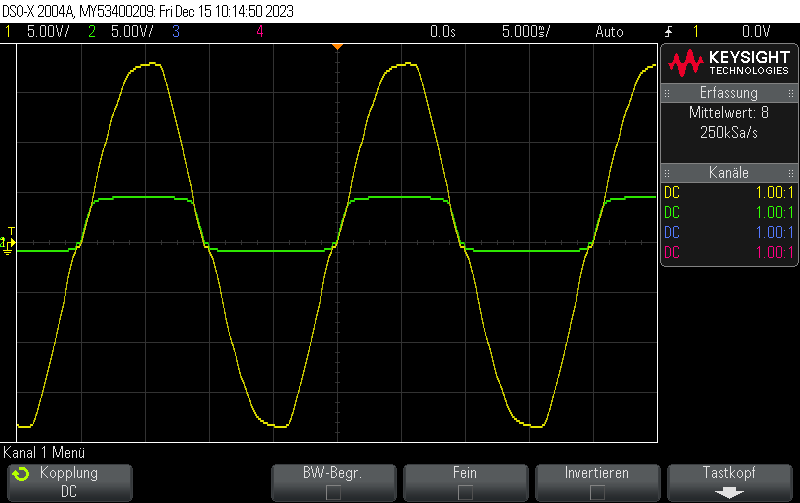
\includegraphics[width=0.6\linewidth]{nudes/Halbleiterdiode/Aufgabe2/a2b1___.png}
    \caption{Screenshot des Oszilloskopes. Dabei ist die gelbe Linie die Eingangsspannung $U_E$ und die grüne Linie die Spannung der Diode $U_{D1}$. }
    \label{fig:mess 2}
\end{figure}

\subsection{Teil 3}
Im dritten Teil folgt der Aufbau laut Abbildung \ref{fig:aufbau 3}. 
Dabei ist das Ziel dieser Aufgabe die Spannungs- und Stromverläufe als zeitabhängige Funktion darzustellen. 
Für jede Konfiguration des Aufbaus wird am Oszilloskop ein Bild und eine CSV-Datei exportiert. 
\\
Dabei ist der Channel 1 des Oszilloskopes (gelb) der Spannungsabfall am Widerstand $R_1$. 
Um die Messung mit den richtigen Vorzeichen zu vollziehen, wird dieser Channel am Oszilloskop invertiert. 
Der Channel 2 (grün) ist die Spannung des Trafos $TR1$. 
Der Channel 3 (blau) ist die Spannung, die über den jeweils eingesetzten Kondensator läuft. 
Der Channel 4 (rot) ist dabei die Lade-Entlade kurve des jeweils eingesetzten Kondensators. 
\\
\\
Die Messungen werden für die Widerstände $R_3 = \infty$ $R_3 = (1500 \pm 10) \Omega$ und $R_3 = (100 \pm 1) \Omega$ mit den Kapazitäten $C_1 = (10.0 \pm 0.1) \mu F$ und $C_1 = (100 \pm 1) \mu F $ durchgeführt. Unsicherheiten implizit angenommen. 

\begin{figure}[H]
    \begin{minipage}[b]{.5\linewidth} % [b] => Ausrichtung an \caption
        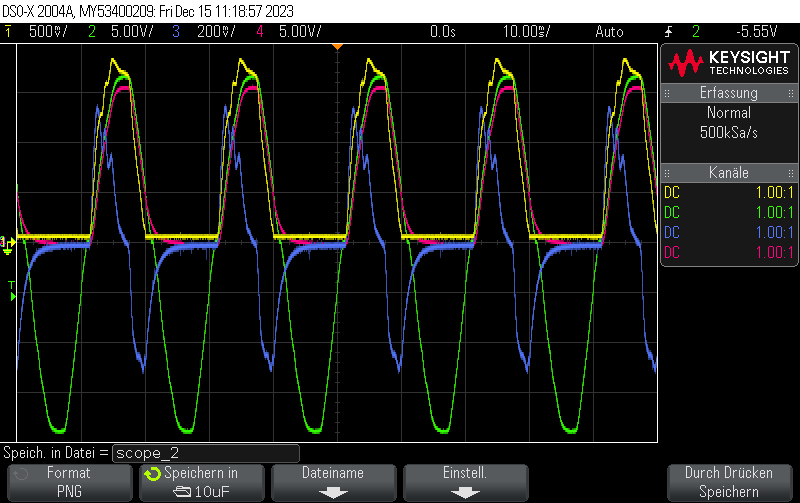
\includegraphics[width=1\linewidth]{nudes/Halbleiterdiode/Aufgabe3/100Ohm/10uF/scope_2.png}
        \caption{$R_3 = 100 \Omega$, $C_1 = 10 \mu F$}
    \end{minipage}
    \hspace{0.01\linewidth}% Abstand zwischen Bilder
    \begin{minipage}[b]{.5\linewidth} % [b] => Ausrichtung an \caption
        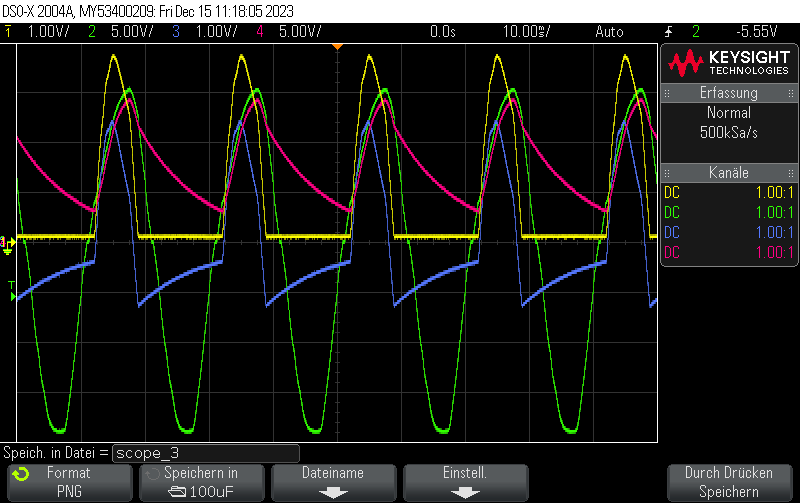
\includegraphics[width=1\linewidth]{nudes/Halbleiterdiode/Aufgabe3/100Ohm/100uF/scope_3.png}
    \caption{$R_3 = 100 \Omega$, $C_1 = 100 \mu F$}
    \end{minipage}
\end{figure}

\begin{figure}[H]
    \begin{minipage}[b]{.5\linewidth} % [b] => Ausrichtung an \caption
        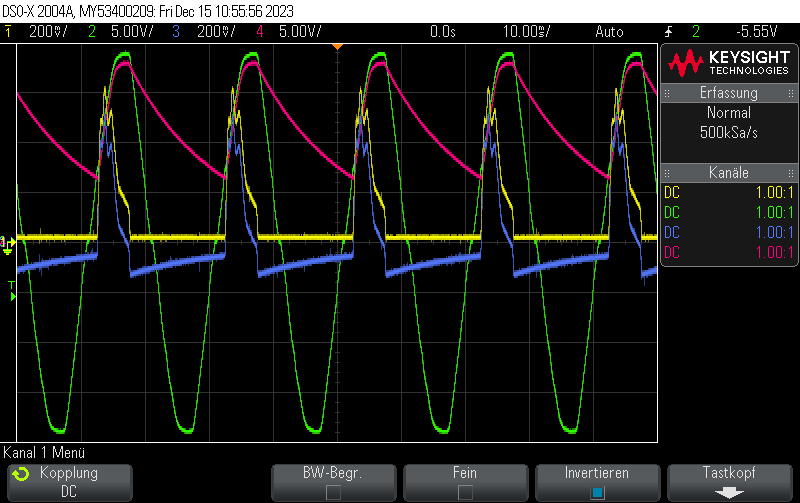
\includegraphics[width=1\linewidth]{nudes/Halbleiterdiode/Aufgabe3/1500Ohm/10uF/a2c2___5.png}
        \caption{$R_3 = 1500 \Omega$, $C_1 = 10 \mu F$}
    \end{minipage}
    \hspace{0.01\linewidth}% Abstand zwischen Bilder
    \begin{minipage}[b]{.5\linewidth} % [b] => Ausrichtung an \caption
        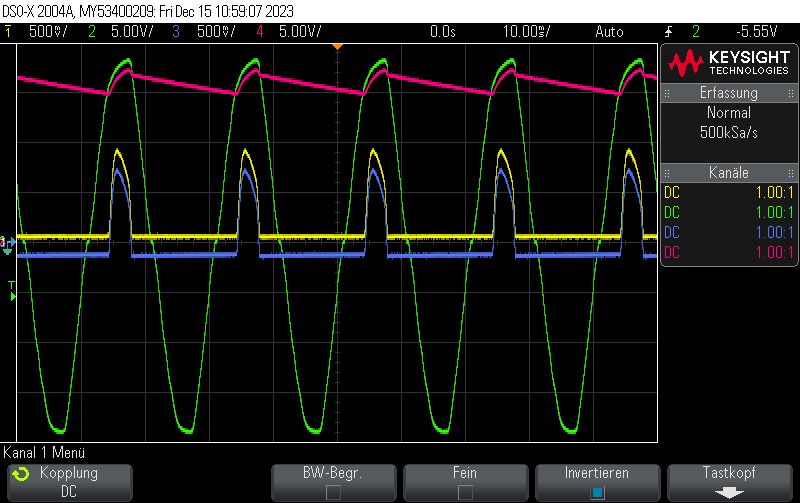
\includegraphics[width=1\linewidth]{nudes/Halbleiterdiode/Aufgabe3/1500Ohm/100uF/a2c2___7.png}
    \caption{$R_3 = 1500 \Omega$, $C_1 = 100 \mu F$}
    \end{minipage}
\end{figure}

\begin{figure}[H]
    \begin{minipage}[b]{.5\linewidth} % [b] => Ausrichtung an \caption
        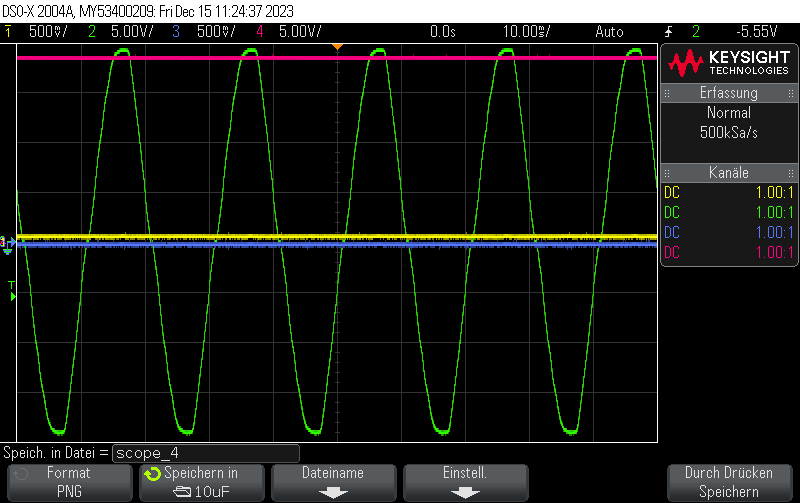
\includegraphics[width=1\linewidth]{nudes/Halbleiterdiode/Aufgabe3/GonzVülOhm/10uF/scope_4.png}
        \caption{$R_3 = \infty$, $C_1 = 10 \mu F$}
    \end{minipage}
    \hspace{0.01\linewidth}% Abstand zwischen Bilder
    \begin{minipage}[b]{.5\linewidth} % [b] => Ausrichtung an \caption
        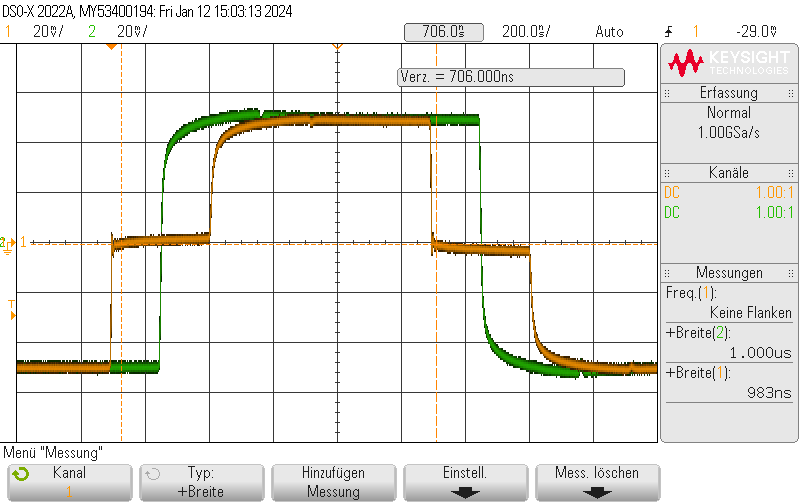
\includegraphics[width=1\linewidth]{nudes/Halbleiterdiode/Aufgabe3/GonzVülOhm/100uF/scope_7.png}
    \caption{$R_3 = \infty$, $C_1 = 100 \mu F$}
    \end{minipage}
\end{figure}

\section{Auswertung und Unsicherheitsanalyse} %Nicht nur zahlen angeben ------------------------------

In der Auswertung werden zur erhöhten Genauigkeit durchgehend ungerundete Werte bis zu den Endergebnissen verwendet und nur zur Darstellung gerundet. \\
Zur Berechnung der Unsicherheiten wird, wenn nicht anders angegeben, die Größtunsicherheitsmethode verwendet.


\section{Diskussion} %diskussion der Unsicherheiten und Ergebnisse und evtl. verlgeich mit Literatur ------------------------------


\section{Zusammenfassung} %klare, übersichtliche vollständige beantwortung der Aufgabenstellung ------------------------------


\printbibliography[heading=bibintoc]
\end{document}
